%[dimension]
Our proposed model consists mainly of two parts: one is an NLU label encoder, and the other is a frame encoder. The two encoders produce a vector for the corresponding part of the input. We use a dot product to compute the similarity score between an NLU label and a frame. The output is a probability distribution over all candidate frames computed by taking softmax of all the similarity scores of the frames. Softmax is a kind of normalization that transforms a real vector into a discrete probability distribution. It is defined as
\begin{equation}\label{eq:softmax}
    \text{softmax}(x)_i = \frac{\exp(x_i)}{\sum_{j = 1}^{n}{\exp(x_j)}} \text{, for } i = 1 \dotsc n\,.
\end{equation}
The high-level overview of the model architecture is in Figure \ref{fig:main}.

\begin{figure}
    \centering
    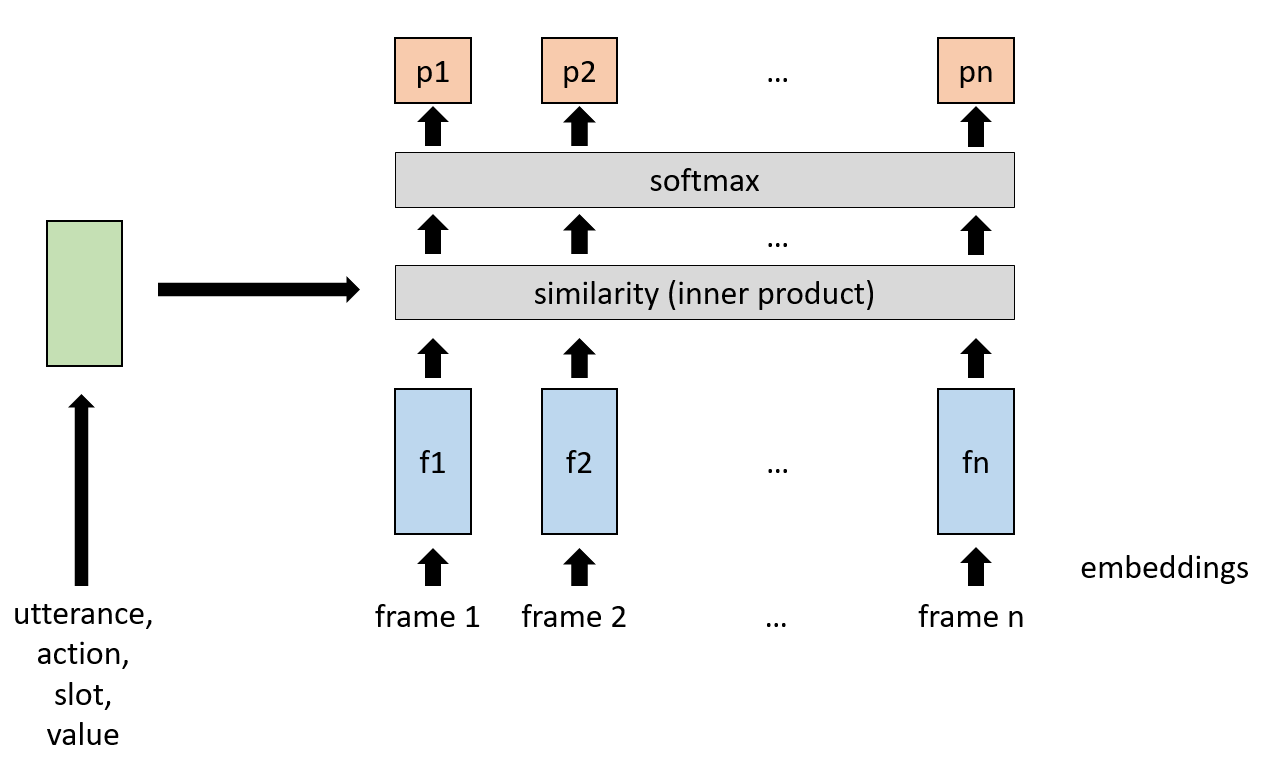
\includegraphics[width=\columnwidth]{figures/main.png}
    \caption[Model architecture]{Model architecture. The green block on the left is NLU label encoder (Figure \ref{fig:nlu-label}). The blue blocks at the bottom are frame encoders (Figure \ref{fig:frame}).}
    \label{fig:main}
\end{figure}

\subsection{Embedding of input}
Both NLU label encoder and frame encoder use text embedding and token embedding to convert structured input into vectors. The embeddings are shared between the two encoders. There are three embeddings: text embedding, act embedding, slot embedding. The act embedding and slot embedding are very similar. We treat each act and slot as a unique token and assign them a trainable embedding vector. The text embedding is used to embed slot values. 

% letter trigram, BERT feature
We use two different text embedding models. The first one, shown in Figure \ref{fig:bert}, is based on a pre-trained BERT \cite{devlin2018bert} feature. We use a uncased 12-layered BERT model\footnote{\url{https://github.com/huggingface/pytorch-transformers}}. The embedding of a slot value is the average of the last layer. We use a linear projection to adjust the dimension of the embedding so that it is compatible with the other part of the model.

\begin{figure}
    \centering
    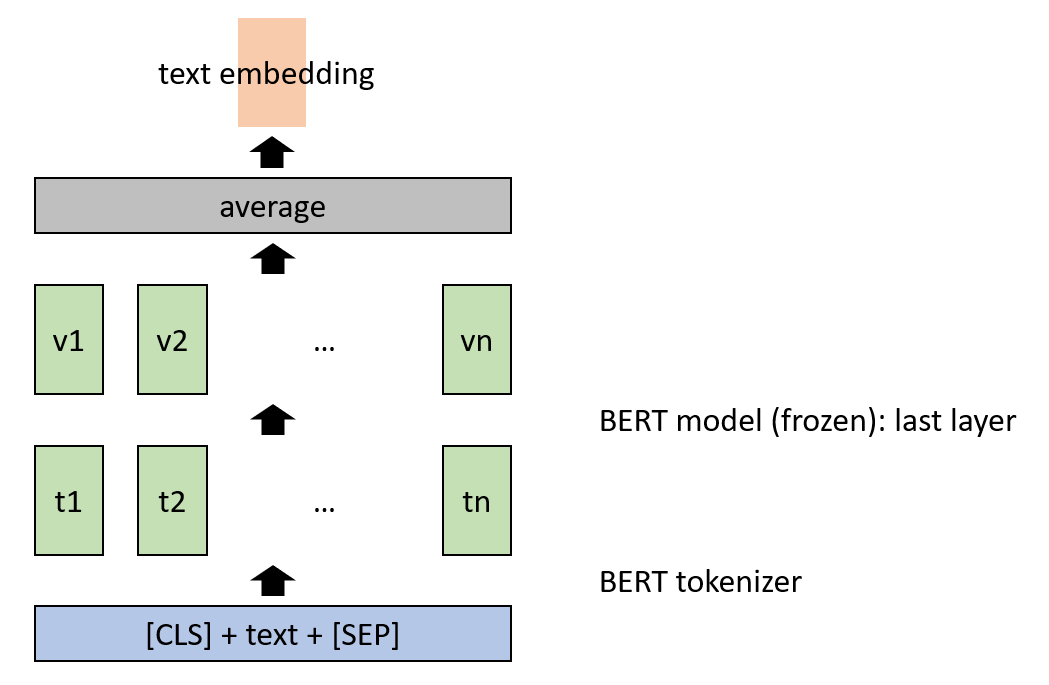
\includegraphics[width=\columnwidth]{figures/bert.png}
    \caption[Text embedding using pre-trained BERT]{Architecture of text embedding using pre-trained BERT.}
    \label{fig:bert}
\end{figure}

The other text embedding is based on letter trigram and RNN (Figure \ref{fig:gru}. We first tokenize the text using nltk's TweetTokenizer\footnote{\url{https://www.nltk.org/}} and split each token into letter trigrams. For example, the list of letter trigram of ``hotel" is ``\#ho", ``hot", ``ote", ``tel", and ``el\#". We assign each trigram to a trainable embedding vector. The embedding of a token is then the sum of embedding of its trigrams. We then use a bidirectional GRU to encode all tokens into one vector. The final embedding is the concatenation of forward and backward hidden state of the GRU.

\begin{figure}
    \centering
    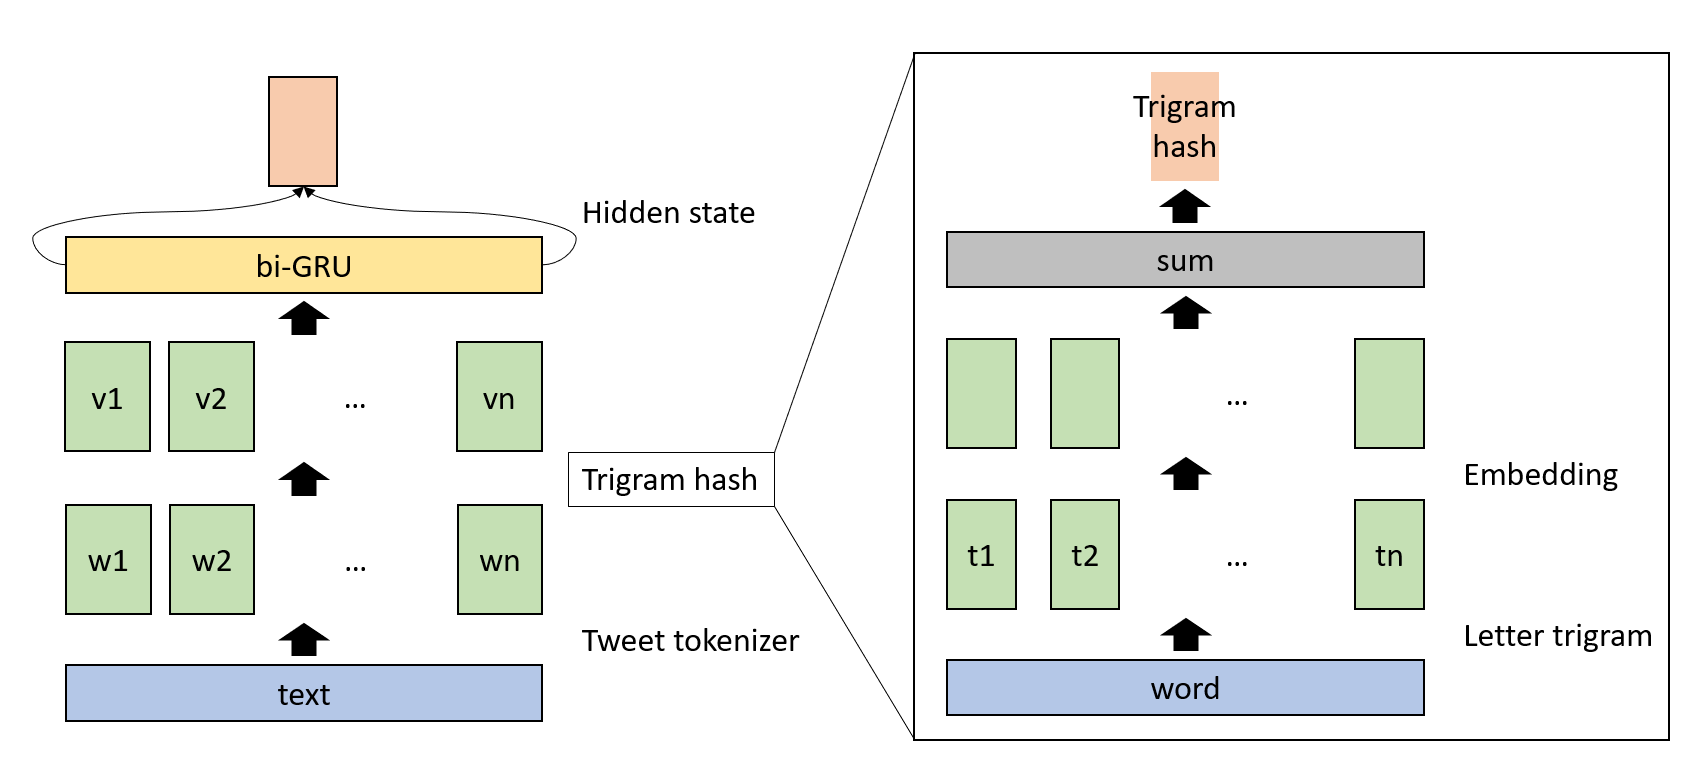
\includegraphics[width=\columnwidth]{figures/lstm.png}
    \caption[Text embedding using letter trigram and GRU]{Architecture of text embedding using letter trigram and GRU.}
    \label{fig:gru}
\end{figure}


\subsection{NLU label encoder}
This encoder takes as input an act embedding, a slot embedding, and a value embedding. We treat them as a sequence of length three and pass it through a bidirectional GRU. We then concatenate the forward and backward hidden state and project it to have a proper dimension. The architecture is in Figure \ref{fig:nlu-label}.

\begin{figure}
    \centering
    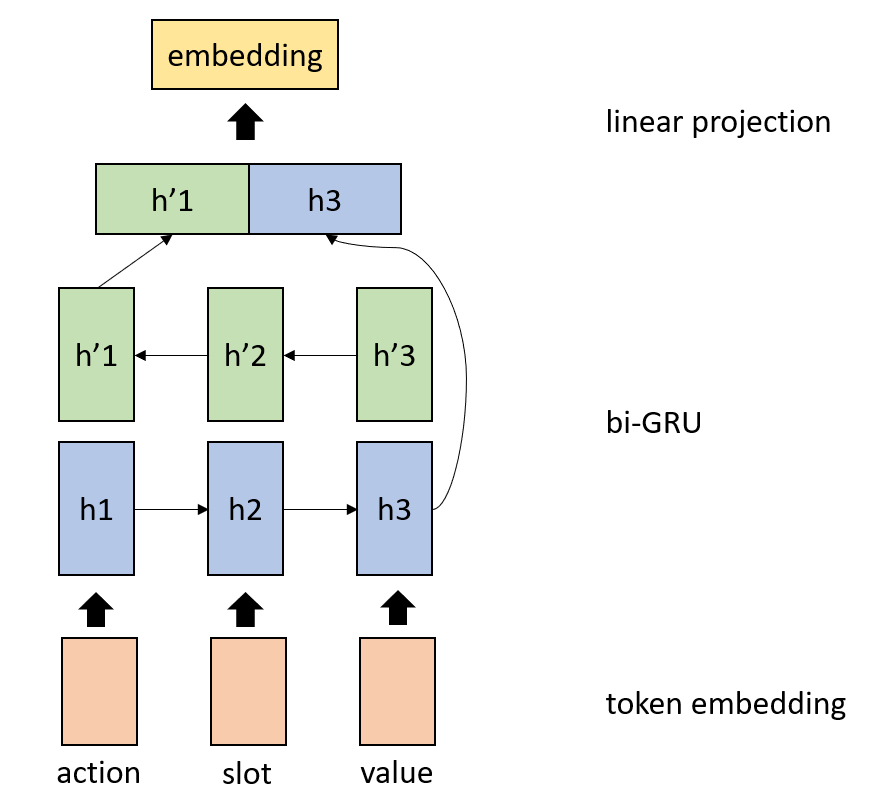
\includegraphics[width=0.7\columnwidth]{figures/utterance.png}
    \caption[NLU label encoder]{Architecture of NLU label encoder.}
    \label{fig:nlu-label}
\end{figure}

\subsection{Frame encoder}
A frame is a list of slot-value pairs. To encode this, we concatenate the slot and value embedding vectors for each slot-value pair and pass the list of concatenated vectors through a bidirectional GRU.

If there is no attention mechanism, we concatenate the forward and backward hidden state of the GRU and use a linear projection to compute the output vector. If an attention mechanism is used, we concatenate the outputs of both direction and project each vector to adjust the dimension. The final output is then the linear combination of the resulting vectors, with coefficients being attention scores normalized by softmax. The architecture with attention mechanism is shown in Figure \ref{fig:frame}.

\begin{figure}
    \centering
    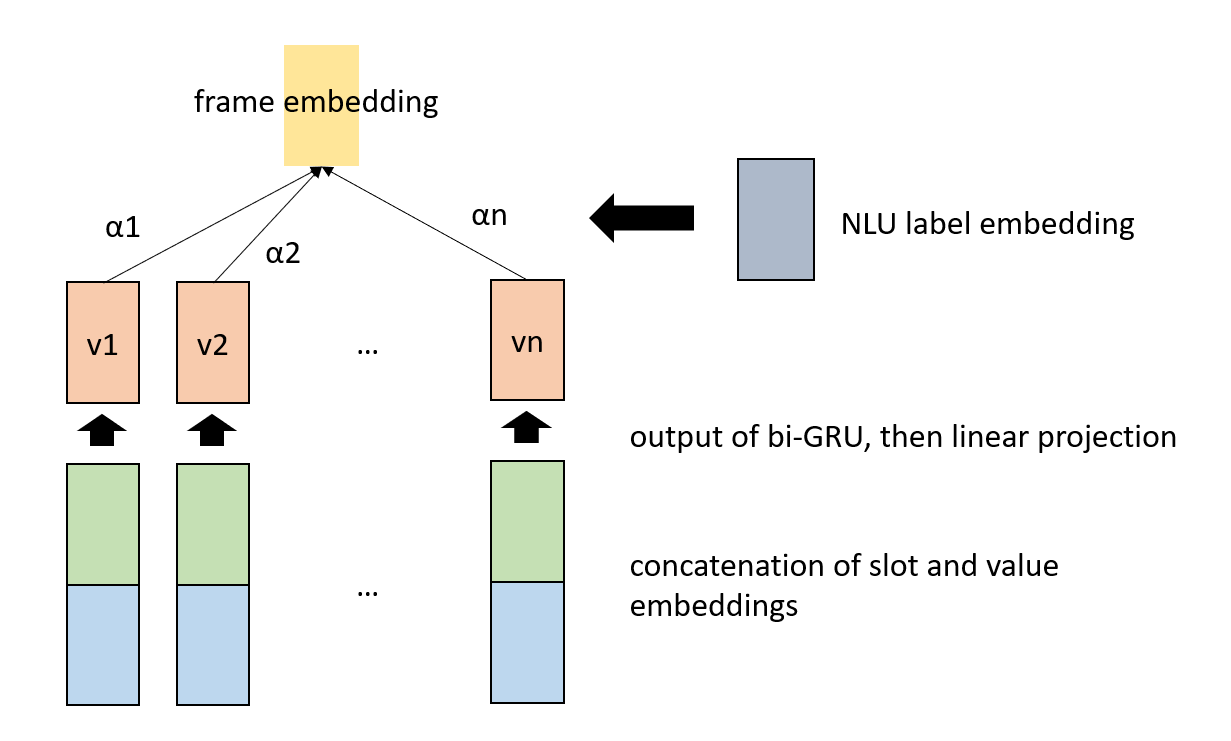
\includegraphics[width=\columnwidth]{figures/frames.png}
    \caption[Frame encoder]{Architecture of frame encoder.}
    \label{fig:frame}
\end{figure}

The detailed formula of each attention mechanism is in Table \ref{tab:att}. In addition to an encoded frame, most of the attention mechanisms we use also take an encoded NLU label as input so that the attention score is adapted for different situations. The only exception is the content-based attention, which computes the score using only the content of slot-values of the given frame.

%[more on attention]
% with query or not

\begin{table}
    \caption[Formulas of attention mechanisms]{Formulas of attention mechanisms. $x$ is the embedding of a NLU label, $y$ is an the embedding of a slot-value pair in a frame, $d_y$ is the dimension of $y$, and $d_k$ is the dimension of $W_ky$. $w$, $W$, $W_k$, $W_q$, and $b$ are trainable parameters.}
    \label{tab:att}
    \centering
    \begin{tabular}{ll}
        \toprule
        Type & Formula for $\alpha$ (attention score) \\
        \midrule
        Content-based & $\tanh(wy+b)$ \\
        Dot-product & $x^Ty$ \\
        Cosine & $x^Ty\ /\ \norm{x}\norm{y}$ \\
        General & $x^TWy$ \\
        Query-key & $(W_qx)^TW_ky$ \\
        Scaled dot-product & $x^Ty / \sqrt{d_y}$ \\
        %Scaled general & $x^TWy / \sqrt{d_y}$ \\
        Scaled query-key & $(W_qx)^TW_ky / \sqrt{d_k}$ \\
        \bottomrule
    \end{tabular}
\end{table}
